\chapter{Demand}
\label{ch:demand}

\section{Introduction}

The demand specifies personal vehicle trips in terms of origins, destinations, and departure times. This chapter discusses the organization of the demand inputs to DTA. All related data files are contained within the \texttt{demand} subfolder of a project. The demand is specified through four files. The \texttt{static\_od.txt} file is a static (time-invariant) trip table that is representative of the static data available to many planning organizations. The \texttt{dynamic\_od.txt} file is a dynamic trip table that specifies the number of trips per \textit{assignment interval} (AST). The \texttt{demand\_profile.txt} file specifies the weight, start time, and duration of each AST. The \texttt{demand.txt} file contains a list of discrete vehicles, each with a specific origin, destination, and departure time. The \texttt{dynamic\_od.txt} file can be generated from the \texttt{static\_od.txt} and the \texttt{demand\_profile.txt} files. The \texttt{demand.txt} file can be generated from the \texttt{dynamic\_od.txt} file and the \texttt{demand\_profile.txt} file.
Vehicle types (i.e. HV, AV, etc.) are specified in the \texttt{static\_od.txt}, \texttt{dynamic\_od.txt}, and \texttt{demand.txt} files. The AVDTA GUI includes methods to generate the \texttt{dynamic\_od.txt} and \texttt{demand.txt} files given appropriate inputs.

\section{Files} 

\subsection{\texttt{static\_od.txt}}
\label{sec:staticod}

The \texttt{static\_od.txt} file is a time-invariant trip table. Each line indicates the number of trips of some type between some origin and destination. The columns are 
\begin{center}
\begin{tabular}{ccccc}
\hline
id & type & origin & destination & demand\\\hline
\end{tabular}
\end{center}
\paragraph*{id} An unique id for the trip table entry. Ids do not have to be consecutive, but must be unique and positive.
\paragraph*{type} The type indicates the type of vehicle, including the driver, engine, and vehicle behavior. The options for types are indicated below:
\begin{center}
\begin{tabular}{lcl}
\hline
Category & type & description \\\hline
Driver & 10 & HV \\
 & 20 & AV\\\hline
Engine & 1 & ICV \\
& 2 & BEV\\\hline
Behavior & 100 & personal vehicle (UE routing)\\
& 500 & transit (fixed route)\\\hline
\end{tabular}
\end{center}
A valid type is the sum of a driver type, an engine type, and a vehicle behavior. Typical types are 111 for HVs and 121 for AVs.

\paragraph*{origin, destination} These are ids of origin and destination zones in the network (see Section \ref{sec:nodes}).
\paragraph*{demand} A floating point number indicating the number of trips of the specified type from the origin to the destination. Duplicate entries (in terms of type, origin, and destination) are accepted.

\subsection{\texttt{dynamic\_od.txt}}
\label{sec:dynamicod}

The \texttt{dynamic\_od.txt} file is like the \texttt{static\_od.txt} file, but with the addition of an AST. Each line The columns are
\begin{center}
\begin{tabular}{cccccc}
\hline
id & type & origin & destination & ast & demand\\\hline
\end{tabular}
\end{center}
\paragraph*{ast} This is the id of an AST from the \texttt{demand\_profile.txt} file (Section \ref{sec:demandprofile}).

The remainder of the columns are the same as in the \texttt{static\_od.txt} file (Section \ref{sec:staticod}). The ids in \texttt{dynamic\_od.txt} do not need to correspond to the ids in \texttt{static\_od.txt}. The \texttt{dynamic\_od.txt} file can be generated within AVDTA from the \texttt{static\_od.txt} and \texttt{demand\_profile.txt} files. The distribution of flow over ASTs is determined by the weights in the \texttt{demand\_profile.txt} file.

\subsection{\texttt{demand\_profile.txt}}
\label{sec:demandprofile}

The \texttt{demand\_profile.txt} file specifies the ASTs. Each line is an individual AST. The columns are
\begin{center}
\begin{tabular}{cccc}
\hline
id & weight & start & duration \\\hline
\end{tabular}
\end{center}
\paragraph*{id} The id must be positive and unique, but does not need to be consecutive.
\paragraph*{weight} This is the proportion of total flow departing within this AST. Proportions will be scaled to sum to 1 if necessary.
\paragraph*{start} This is the starting time of the AST, measured in seconds from the beginning of the simulation period.
\paragraph*{duration} This is the duration of the AST. A typical value is 900 (s).


\subsection{\texttt{demand.txt}}
Each line in the \texttt{demand.txt} file is an individual vehicle trip. The columns are
\begin{center}
\begin{tabular}{cccccc}
\hline
id & type & origin & dest & dtime & vot \\\hline
\end{tabular}
\end{center}
\paragraph*{id} The unique vehicle id. Ids must be positive and unique but do not have to be consecutive.
\paragraph*{type} The vehicle type (see Section \ref{sec:staticod} for a list of types).
\paragraph*{origin, dest} The ids of the origin and destination zones for the vehicle (see Section \ref{sec:nodes}).
\paragraph*{dtime} The departure time of the vehicle, measured in seconds from the start of the simulation period.
\paragraph*{vot} The value of time of the vehicle. This is used in certain control policies, such as auctions for reservations. Values of time must be non-negative.


\section{GUI}
This section describes how to interact with the demand through the AVDTA GUI. The ``demand'' tab contains all demand interactions. 

\subsection{Import demand}
The left hand side contains options to import demand from other sources. The first option is to import the demand from another DTA project. This will copy all demand files from the specified project, overwriting any demand files in the current project. Click on the text field to select the project.
\begin{center}
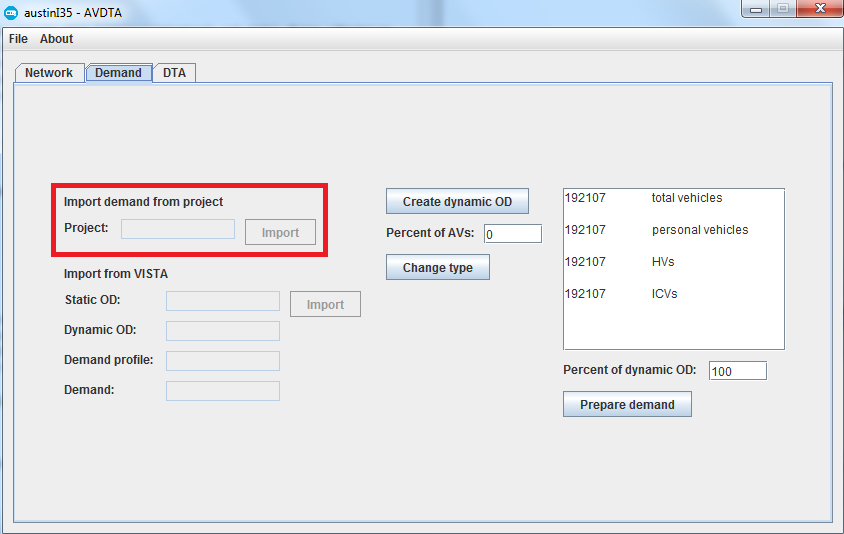
\includegraphics[width=0.8\textwidth]{images/demand1.png}
\end{center}

The second option is to import demand from VISTA. This requires the \texttt{static\_od}, \texttt{dynamic\_od}, \texttt{demand\_profile}, and \texttt{demand} tables from the VISTA database. Copy them into text files, and select the text files by clicking on the text fields. Note that the file format of AVDTA is not the same as the file format of VISTA, so using the GUI to import demand is recommended.
\begin{center}
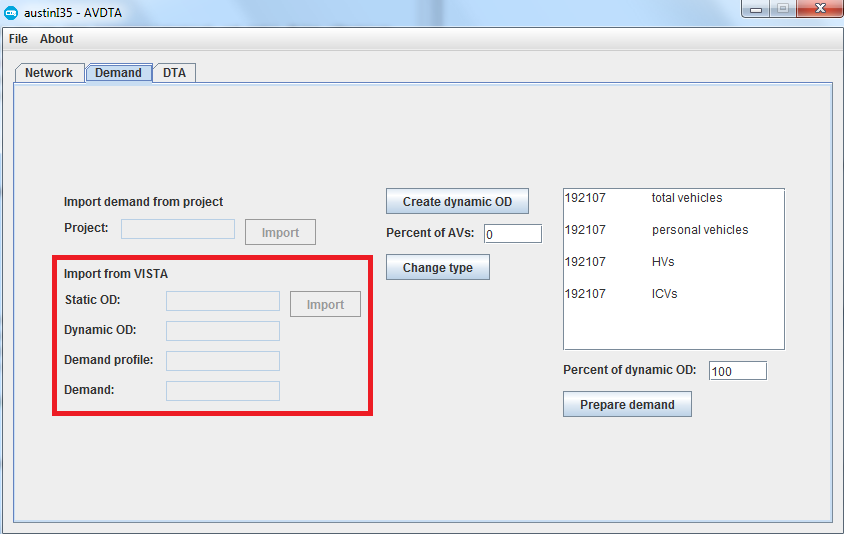
\includegraphics[width=0.8\textwidth]{images/demand2.png}
\end{center}

\subsection{Creating demand}
The middle section includes options to change the \texttt{dynamic\_od.txt} file. The first button will generate the \texttt{dynamic\_od.txt} file based on the \texttt{static\_od.txt} and the \texttt{demand\_profile.txt} files, as discussed in Section \ref{sec:dynamicod}. 
\begin{center}
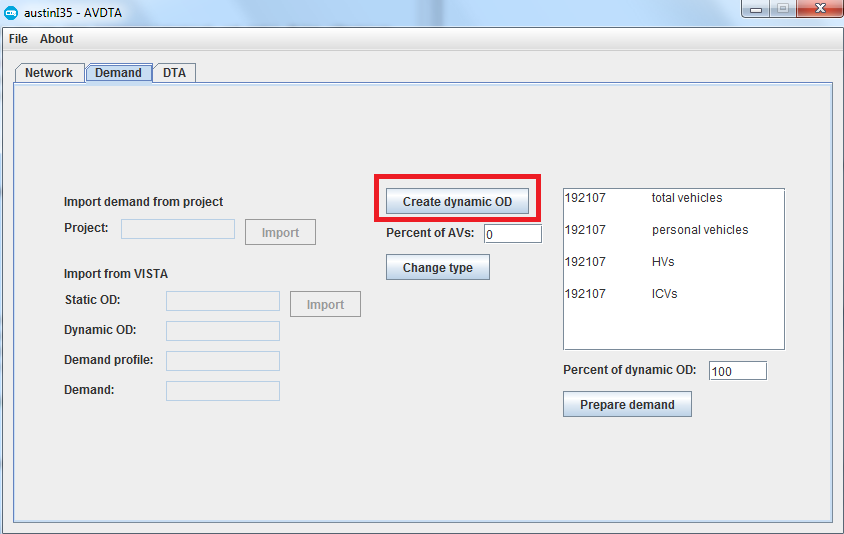
\includegraphics[width=0.8\textwidth]{images/demand3.png}
\end{center}

The second option will change the type of vehicles to 111 for HVs or 121 for AVs (see Section \ref{sec:staticod} for types) in the \texttt{dynamic\_od.txt} file based on the specified percent of AVs. 
\begin{center}
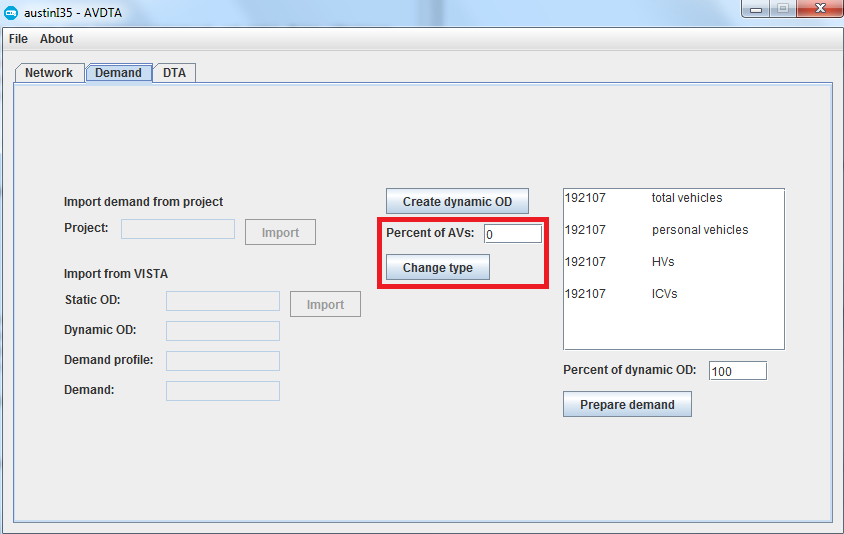
\includegraphics[width=0.8\textwidth]{images/demand3b.png}
\end{center}

The right hand side describes the individual vehicle trips. The text area lists the total numbers of vehicles, then breaks down the numbers of vehicles by type (driver, engine, and behavior). Click the ``prepare demand'' button to generate the \texttt{demand.txt} file from the \texttt{dynamic\_od.txt} and \texttt{demand\_profile.txt} files. You can also scale the percent of demand. 

Preparing demand uses a random number generator when the number of trips is not an integer. If $d$ is the number of vehicle trips in \texttt{dynamic\_od.txt}, prepare demand will create either $\lfloor d\rfloor$ or $\lceil d\rceil$ trips depending on the outcome of the random number generator.
\begin{center}
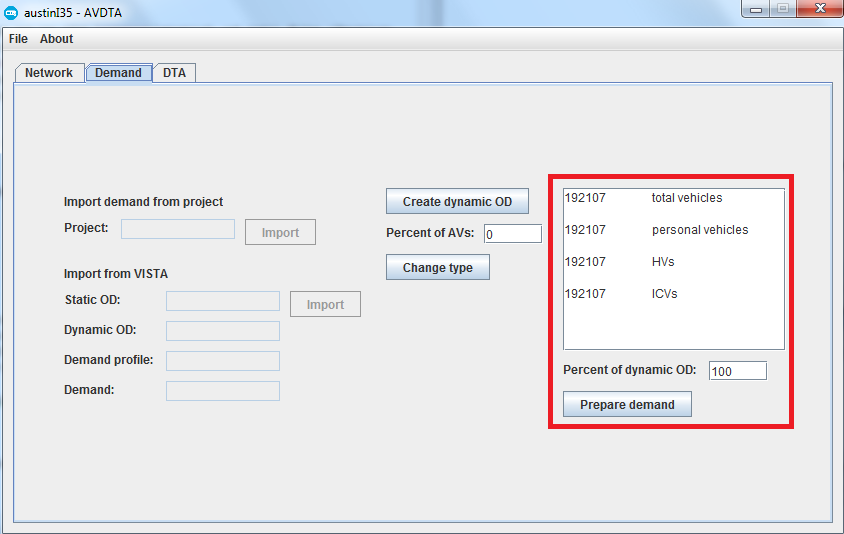
\includegraphics[width=0.8\textwidth]{images/demand4.png}
\end{center}